% Provenance (never printed): cycle 2 "Questionner l'espace et le temps"
% (the globe, the continents and the oceans, reading a world map); see
% sources/book1/PROVENANCE.md. Book 1, grade 3, chapter 2.
\chapter{El globo terráqueo: continentes y océanos}\label{ch:g3:continents-and-oceans}

En el aula de Lena hay un \omterm{def:g3:continents-and-oceans:globe}{globo terráqueo} sobre un soporte. Lena cierra los
ojos, lo hace girar con un dedo y lo detiene con la punta del dedo. Abre
los ojos: su dedo está sobre el azul, en medio de un \omterm{def:g2:water-on-earth:ocean}{océano}. Lo intenta otra
vez: azul de nuevo. A la tercera, cae sobre el verde amarillento, en algún
lugar del centro de África.

Lena sigue jugando y va contando. Su dedo se para mucho más a menudo sobre
el \omterm{def:g2:water-on-earth:ocean}{mar} que sobre la tierra. ¿Por qué? ¿Y qué son todas esas formas de
tierra y de agua que giran bajo su dedo?

\begin{omfigure}
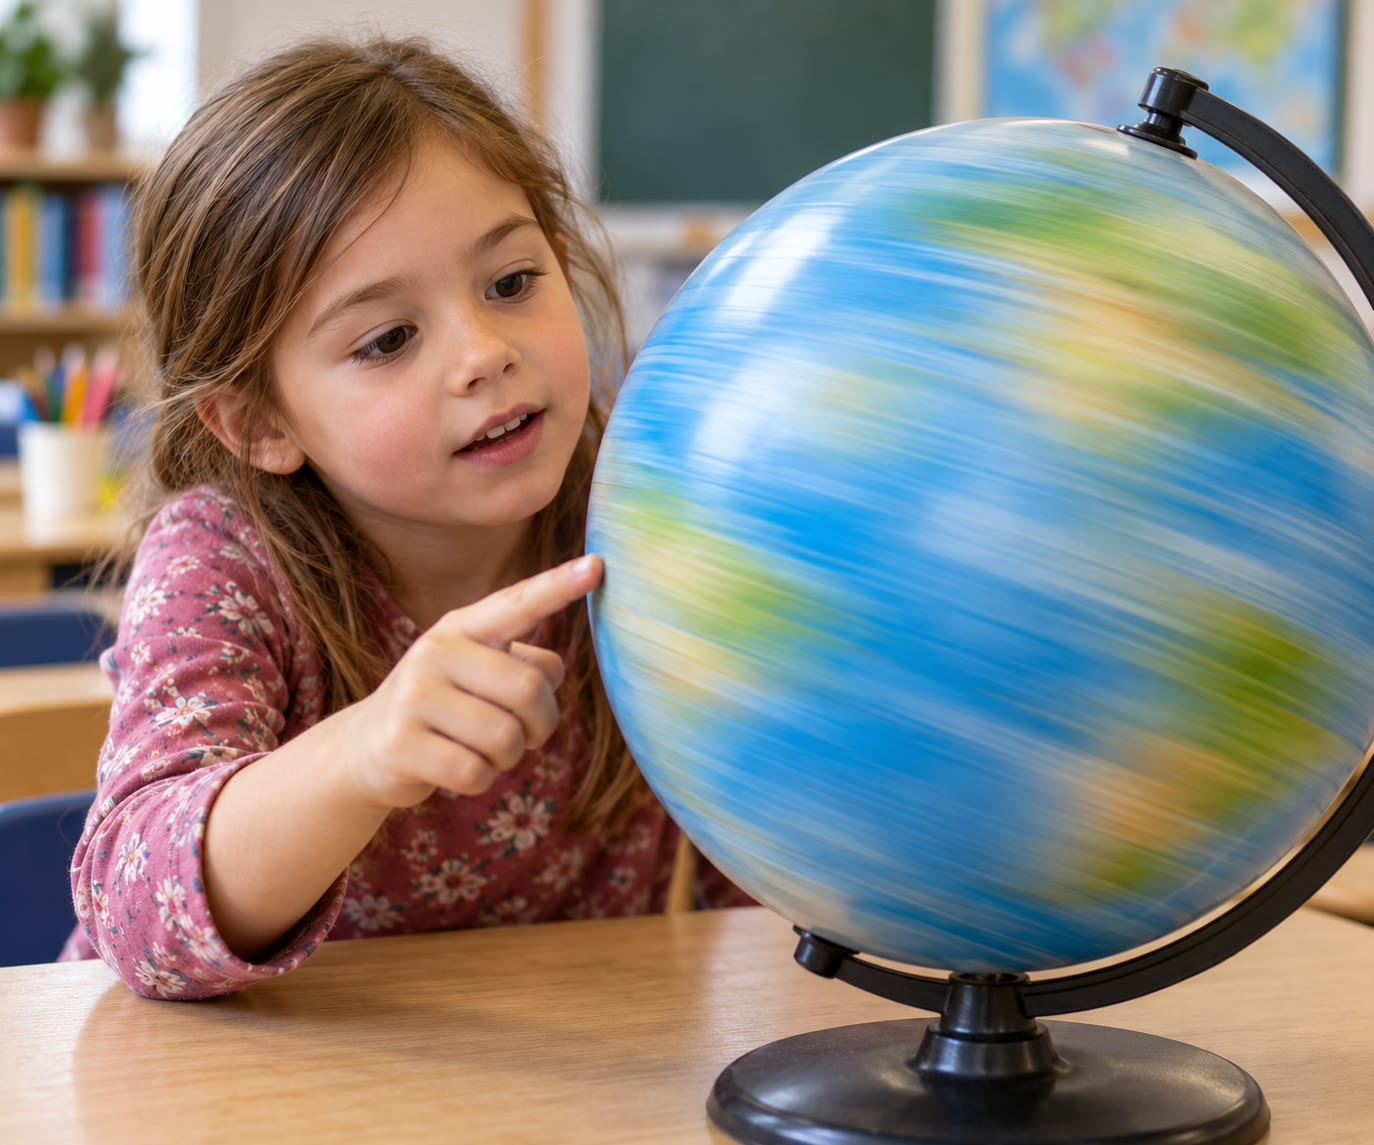
\includegraphics[width=0.6\linewidth]{images/book1/ai/g3-spinning-globe.jpg}

{\small Un \omterm{def:g3:continents-and-oceans:globe}{globo terráqueo} que gira sobre su soporte: la tierra y el \omterm{def:g2:water-on-earth:ocean}{mar}
pasan bajo el dedo.}
\end{omfigure}

\begin{recall}
Casi toda la Tierra está cubierta de \omterm{def:g2:water-on-earth:salt-fresh}{agua salada}: unos 71 cuadrados de
cada 100 en la cuadrícula del \cref{ch:g2:water-on-earth}. Un \omterm{def:g2:water-on-earth:ocean}{océano} es una
extensión muy grande de \omterm{def:g2:water-on-earth:salt-fresh}{agua salada} entre las masas de tierra; un \omterm{def:g2:water-on-earth:ocean}{mar} es una
más pequeña, en el borde de un \omterm{def:g2:water-on-earth:ocean}{océano}. Un \omterm{def:g2:drawing-to-map:map}{mapa} es un dibujo de un lugar
visto desde arriba, hecho más pequeño (\cref{ch:g2:drawing-to-map}). Los
libros de física cuentan cómo la Tierra gira sobre sí misma una vez al día,
lo que nos da el día y la noche.
\end{recall}

\section{El globo terráqueo, una pequeña maqueta de la Tierra redonda}

La Tierra es redonda, como una pelota enorme. Desde el suelo no podemos ver
su forma, porque es demasiado grande: estemos donde estemos, el suelo parece
llano. Pero los astronautas que viajaron lejos de la Tierra la vieron
entera, una pelota azul y redonda en el cielo negro (la fotografía del
principio del \cref{ch:g2:water-on-earth}).

Para ver la Tierra entera en un aula, la hacemos pequeña.

\begin{definition}[Globo terráqueo]\label{def:g3:continents-and-oceans:globe}
Un \emph{globo terráqueo}\index{globo terraqueo@globo terráqueo} es una
maqueta de la Tierra: una bola en la que están dibujados la tierra y los
\omterm{def:g2:water-on-earth:ocean}{océanos} con las mismas formas que en la Tierra real, solo que muchísimo más
pequeños.
\end{definition}

Un \omterm{def:g3:continents-and-oceans:globe}{globo terráqueo} es la mejor imagen de la Tierra, porque tiene la forma
correcta: redonda. Pero, igual que con la Tierra real, solo podemos ver una
mitad de cada vez. Para ver la otra mitad, lo hacemos girar.

\begin{omfigure}
\begin{tikzpicture}
\begin{axis}[name=atl, hide axis, axis equal image, scale only axis,
    width=6.2cm, xmin=-1.05, xmax=1.05, ymin=-1.05, ymax=1.05, clip=false]
  \fill[omSea] (axis cs:0,0) circle[radius=1];
  \addplot[fill=omHypsLandA!85!black, draw=black!45, line width=0.2pt]
    table {figdata/out/grade-3-globe-atlantic-land.dat};
  \addplot[black!60, dashed, line width=0.5pt]
    table {figdata/out/grade-3-globe-atlantic-equator.dat};
  \addplot[only marks, mark=*, mark size=1.4pt, black]
    table[x=x, y=y] {figdata/out/grade-3-globe-atlantic-poles.dat};
    % the names of figdata/out/grade-3-globe-atlantic-labels.dat, in Spanish
  \node[font=\scriptsize, align=center, fill=white, fill opacity=0.7, text opacity=1, inner sep=1pt, rounded corners=1pt] at (axis cs:-0.683,0.636) {América\\del Norte};
  \node[font=\scriptsize, align=center, fill=white, fill opacity=0.7, text opacity=1, inner sep=1pt, rounded corners=1pt] at (axis cs:-0.561,-0.408) {América\\del Sur};
  \node[font=\scriptsize, align=center, fill=white, fill opacity=0.7, text opacity=1, inner sep=1pt, rounded corners=1pt] at (axis cs:0.396,0.639) {Europa};
  \node[font=\scriptsize, align=center, fill=white, fill opacity=0.7, text opacity=1, inner sep=1pt, rounded corners=1pt] at (axis cs:0.704,-0.098) {África};
  \node[font=\scriptsize, align=center, fill=white, fill opacity=0.7, text opacity=1, inner sep=1pt, rounded corners=1pt] at (axis cs:-0.209,0.128) {océano\\Atlántico};
  \draw[black!70, line width=0.8pt] (axis cs:0,0) circle[radius=1];
  \node[font=\scriptsize, anchor=south] at (axis cs:0,0.97) {Polo Norte};
\end{axis}
\begin{axis}[at={(atl.east)}, anchor=west, xshift=0.6cm, hide axis,
    axis equal image, scale only axis,
    width=6.2cm, xmin=-1.05, xmax=1.05, ymin=-1.05, ymax=1.05, clip=false]
  \fill[omSea] (axis cs:0,0) circle[radius=1];
  \addplot[fill=omHypsLandA!85!black, draw=black!45, line width=0.2pt]
    table {figdata/out/grade-3-globe-pacific-land.dat};
  \addplot[black!60, dashed, line width=0.5pt]
    table {figdata/out/grade-3-globe-pacific-equator.dat};
    % the names of figdata/out/grade-3-globe-pacific-labels.dat, in Spanish
  \node[font=\scriptsize, align=center, fill=white, fill opacity=0.7, text opacity=1, inner sep=1pt, rounded corners=1pt] at (axis cs:-0.754,-0.391) {Australia};
  \node[font=\scriptsize, align=center, fill=white, fill opacity=0.7, text opacity=1, inner sep=1pt, rounded corners=1pt] at (axis cs:0.258,0.087) {océano\\Pacífico};
  \draw[black!70, line width=0.8pt] (axis cs:0,0) circle[radius=1];
\end{axis}
\end{tikzpicture}

{\small El \omterm{def:g3:continents-and-oceans:globe}{globo terráqueo} visto por dos lados. A la izquierda, el lado del
\omterm{def:g2:water-on-earth:ocean}{océano} Atlántico, con América, Europa y África. A la derecha, el otro lado,
el del \omterm{def:g2:water-on-earth:ocean}{océano} Pacífico, con Australia en su borde. La línea discontinua es
el \omterm{def:g3:continents-and-oceans:equator}{ecuador}. Costas: Natural Earth (dominio público).}
\label{fig:g3:continents-and-oceans:globes}
% ledger: data:ne-land
\end{omfigure}

\begin{remark}[Dos mitades muy distintas]\label{rem:g3:continents-and-oceans:halves}
Mira los dos dibujos. A la izquierda, la tierra ocupa unas 4 partes de cada
10 del dibujo. A la derecha, solo 1 parte de cada 10: el lado de la Tierra
que da al Pacífico es casi todo agua. Si el dedo de Lena se para en ese
lado del \omterm{def:g3:continents-and-oceans:globe}{globo}, casi siempre caerá en el \omterm{def:g2:water-on-earth:ocean}{mar}.
\end{remark}

\section{El ecuador, los polos y los dos hemisferios}

Un \omterm{def:g3:continents-and-oceans:globe}{globo terráqueo} gira sobre una varilla que lo atraviesa de arriba abajo.
La Tierra real no tiene varilla, pero también gira alrededor de una línea
que pasa por su centro. Los dos lugares por donde esa línea sale de la
Tierra tienen nombre.

\begin{definition}[Polo]\label{def:g3:continents-and-oceans:poles}
El \emph{Polo Norte}\index{Polo Norte} y el \emph{Polo
Sur}\index{Polo Sur} son los dos puntos situados arriba del todo y abajo
del todo en la Tierra, por donde sale la línea alrededor de la cual gira la
Tierra. Cada uno de ellos es un \emph{polo}\index{polo}. En un \omterm{def:g3:continents-and-oceans:globe}{globo
terráqueo}, el Polo Norte está arriba.
\end{definition}

\begin{definition}[Ecuador y hemisferio]\label{def:g3:continents-and-oceans:equator}
El \emph{ecuador}\index{ecuador} es una línea imaginaria que da toda la
vuelta a la Tierra, justo a medio camino entre el \omterm{def:g3:continents-and-oceans:poles}{Polo Norte} y el \omterm{def:g3:continents-and-oceans:poles}{Polo Sur}.
Corta la Tierra en dos mitades, cada una llamada
\emph{hemisferio}\index{hemisferio}: el \emph{hemisferio
norte}\index{hemisferio norte}, del lado del \omterm{def:g3:continents-and-oceans:poles}{Polo Norte}, y el
\emph{hemisferio sur}\index{hemisferio sur}, del lado del \omterm{def:g3:continents-and-oceans:poles}{Polo Sur}.
\end{definition}

El \omterm{def:g3:continents-and-oceans:equator}{ecuador} no está pintado en el suelo: nadie puede verlo en una playa ni
en un bosque. Se dibuja en los \omterm{def:g3:continents-and-oceans:globe}{globos terráqueos} y en los \omterm{def:g2:drawing-to-map:map}{mapas} para
ayudarnos a orientarnos.

\begin{omfigure}
\begin{tikzpicture}[font=\small]
  % globe outline
  \fill[omSea!70] (0,0) circle (2.2);
  % northern hemisphere tinted
  \begin{scope}
    \clip (0,0) circle (2.2);
    \fill[yellow!25, opacity=0.8] (-2.3,0) -- (-2.3,2.3) -- (2.3,2.3) -- (2.3,0)
      arc[start angle=0, end angle=-180, x radius=2.3, y radius=0.45] -- cycle;
  \end{scope}
  \draw[black!70, line width=0.8pt] (0,0) circle (2.2);
  % equator: front half solid, back half dashed
  \draw[red!70!black, line width=1.2pt] (-2.2,0) arc[start angle=180, end angle=360, x radius=2.2, y radius=0.4];
  \draw[red!70!black, line width=0.8pt, dashed] (2.2,0) arc[start angle=0, end angle=180, x radius=2.2, y radius=0.4];
  % axis and poles
  \draw[black!60, line width=0.6pt] (0,2.2) -- (0,2.75);
  \draw[black!60, line width=0.6pt] (0,-2.2) -- (0,-2.75);
  \draw[black!60, line width=0.6pt, dotted] (0,2.2) -- (0,-2.2);
  \fill (0,2.2) circle (2.2pt);
  \fill (0,-2.2) circle (2.2pt);
  \node[anchor=west] at (0.15,2.6) {Polo Norte};
  \node[anchor=west] at (0.15,-2.6) {Polo Sur};
  % labels
  \node[anchor=west] at (2.6,0) {ecuador};
  \draw[black!60] (2.55,0) -- (2.05,-0.15);
  \node[anchor=west, align=left] at (2.6,1.4) {hemisferio\\norte};
  \draw[black!60] (2.55,1.4) -- (1.5,1.2);
  \node[anchor=west, align=left] at (2.6,-1.4) {hemisferio\\sur};
  \draw[black!60] (2.55,-1.4) -- (1.5,-1.2);
\end{tikzpicture}

{\small El \omterm{def:g3:continents-and-oceans:equator}{ecuador} corta la Tierra en dos \omterm{def:g3:continents-and-oceans:equator}{hemisferios}. El \omterm{def:g3:continents-and-oceans:equator}{hemisferio norte}
(coloreado) está del lado del \omterm{def:g3:continents-and-oceans:poles}{Polo Norte}; el \omterm{def:g3:continents-and-oceans:equator}{hemisferio sur}, del lado del
\omterm{def:g3:continents-and-oceans:poles}{Polo Sur}.}
\label{fig:g3:continents-and-oceans:hemispheres}
\end{omfigure}

\begin{example}[Calor cerca del ecuador, frío cerca de los polos]\label{ex:g3:continents-and-oceans:hot-cold}
Las tierras cercanas al \omterm{def:g3:continents-and-oceans:equator}{ecuador} son cálidas todo el año: allí crecen las
grandes selvas tropicales. Las tierras cercanas a los \omterm{def:g3:continents-and-oceans:poles}{polos} son frías todo
el año, y buena parte de ellas está cubierta de hielo. En un curso
posterior aprenderás por qué es así; por ahora, recuerda: cuanto más cerca
de un \omterm{def:g3:continents-and-oceans:poles}{polo}, más frío.
\end{example}

\section{Siete continentes y cinco océanos}

En un \omterm{def:g3:continents-and-oceans:globe}{globo terráqueo}, la tierra no está repartida en trocitos por todas
partes. Casi toda está reunida en unas pocas masas muy grandes.

\begin{definition}[Continente]\label{def:g3:continents-and-oceans:continent}
Un \emph{continente}\index{continente} es una de las masas de tierra muy
grandes de la Tierra, junto con las islas cercanas a ella.
\end{definition}

Lo más habitual es contar siete \omterm{def:g3:continents-and-oceans:continent}{continentes}. Del más grande al más pequeño,
son: Asia, África, América del Norte, América del Sur, la Antártida, Europa
y Australia.
% ledger: natgeo:seven-continents

\begin{center}\small
\begin{tabular}{rlll}
\hline
Puesto & \omterm{def:g3:continents-and-oceans:continent}{Continente} & \omterm{def:g3:continents-and-oceans:equator}{Hemisferio} & Algo sobre él \\
\hline
1 & Asia & sobre todo norte & el más grande \\
2 & África & los dos & el \omterm{def:g3:continents-and-oceans:equator}{ecuador} cruza su centro \\
3 & América del Norte & norte & llega muy lejos hacia el norte \\
4 & América del Sur & sobre todo sur & el \omterm{def:g3:continents-and-oceans:equator}{ecuador} cruza su norte \\
5 & Antártida & sur & alrededor del \omterm{def:g3:continents-and-oceans:poles}{Polo Sur}, bajo el hielo \\
6 & Europa & norte & unida a Asia por su lado este \\
7 & Australia & sur & el más pequeño \\
\hline
\end{tabular}
\end{center}

\begin{remark}[¿Dónde termina un continente?]\label{rem:g3:continents-and-oceans:where}
Algunos \omterm{def:g3:continents-and-oceans:continent}{continentes} están rodeados de \omterm{def:g2:water-on-earth:ocean}{mar} por todos lados, como Australia o
la Antártida. Otros se tocan: Europa y Asia son una sola masa de tierra, y
la gente eligió dónde trazar la línea entre ellas. Por eso hay quien cuenta
seis \omterm{def:g3:continents-and-oceans:continent}{continentes}, o incluso menos.
\end{remark}

Entre los \omterm{def:g3:continents-and-oceans:continent}{continentes} están los \omterm{def:g2:water-on-earth:ocean}{océanos}. Hay cinco. El más grande es el
\emph{\omterm{def:g2:water-on-earth:ocean}{océano} Pacífico}; después vienen el \emph{\omterm{def:g2:water-on-earth:ocean}{océano} Atlántico}, el
\emph{\omterm{def:g2:water-on-earth:ocean}{océano} Índico}, el \emph{\omterm{def:g2:water-on-earth:ocean}{océano} Austral}, alrededor de la Antártida,
y el más pequeño, el \emph{\omterm{def:g2:water-on-earth:ocean}{océano} Ártico}, alrededor del \omterm{def:g3:continents-and-oceans:poles}{Polo Norte}. Durante
mucho tiempo se contaron solo cuatro; hoy la mayoría de los países cuentan
el \omterm{def:g2:water-on-earth:ocean}{océano} Austral como el quinto.
% ledger: nos:five-oceans, nos:pacific-largest, oer:arctic-smallest

\begin{example}[¿Cómo de grande es el Pacífico?]\label{ex:g3:continents-and-oceans:pacific}
El \omterm{def:g2:water-on-earth:ocean}{océano} Pacífico es tan grande que todos los \omterm{def:g3:continents-and-oceans:continent}{continentes} juntos cabrían
dentro de él. Contiene más de la mitad de toda el agua de los \omterm{def:g2:water-on-earth:ocean}{océanos} de la
Tierra. Por eso el \omterm{def:g3:continents-and-oceans:globe}{globo} de la derecha, en la primera sección de este
capítulo, parece casi todo azul.
% ledger: nos:pacific-largest
\end{example}

\begin{method}[Nombrar el océano entre dos continentes]\label{met:g3:continents-and-oceans:between}
Para saber qué \omterm{def:g2:water-on-earth:ocean}{océano} hay entre dos \omterm{def:g3:continents-and-oceans:continent}{continentes}, pon un dedo sobre cada uno
de ellos en el \omterm{def:g3:continents-and-oceans:globe}{globo terráqueo} y gíralo hasta que veas los dos. El \omterm{def:g2:water-on-earth:ocean}{océano}
que cruza tu mirada para ir de un dedo al otro es el que está entre ellos.
En un \omterm{def:g3:continents-and-oceans:globe}{globo} suele haber dos caminos: toma el más corto.
\end{method}

\begin{example}[África y Australia]\label{ex:g3:continents-and-oceans:africa-australia}
Si vamos de África hacia el este, hacia Australia, cruzamos el \omterm{def:g2:water-on-earth:ocean}{océano}
Índico. Si vamos de Europa hacia el oeste, hasta América del Norte, cruzamos
el \omterm{def:g2:water-on-earth:ocean}{océano} Atlántico. Si vamos de Asia hacia el este, hasta América del
Norte, cruzamos el \omterm{def:g2:water-on-earth:ocean}{océano} Pacífico.
\end{example}

\section{Un mapamundi es un globo aplanado}

Un \omterm{def:g3:continents-and-oceans:globe}{globo terráqueo} es redondo, así que no es fácil de llevar, y nunca
podemos verlo entero de una vez. Un \omterm{def:g2:drawing-to-map:map}{mapa} en una hoja de papel muestra la
Tierra entera de una sola mirada.

\begin{definition}[Mapamundi]\label{def:g3:continents-and-oceans:world-map}
Un \emph{mapamundi}\index{mapamundi} es un \omterm{def:g2:drawing-to-map:map}{mapa} de la Tierra entera dibujado
en plano sobre una hoja de papel o una pantalla, con todos los \omterm{def:g3:continents-and-oceans:continent}{continentes}
y todos los \omterm{def:g2:water-on-earth:ocean}{océanos} en una sola imagen.
\end{definition}

\begin{omfigure}
\begin{tikzpicture}
\begin{axis}[ommap, width=\linewidth, xtick=\empty, ytick={0},
    yticklabels={ecuador}, grid=none, clip=true]
  \addplot[fill=omHypsLandA!85!black, draw=black!45, line width=0.2pt]
    table {figdata/out/shared-geo-land.dat};
  \draw[black!60, dashed, line width=0.5pt] (axis cs:-180,0) -- (axis cs:180,0);
  \begin{scope}[every node/.style={font=\scriptsize, align=center}]
    \node at (axis cs:-102,47) {América\\del Norte};
    \node at (axis cs:-60,-12) {América\\del Sur};
    \node at (axis cs:17,52) {Europa};
    \node at (axis cs:20,6) {África};
    \node at (axis cs:92,48) {Asia};
    \node at (axis cs:134,-24) {Australia};
    \node at (axis cs:40,-80) {Antártida};
  \end{scope}
  \begin{scope}[every node/.style={font=\scriptsize\itshape, align=center, text=omSea!35!black}]
    \node at (axis cs:-145,8) {océano\\Pacífico};
    \node at (axis cs:165,12) {océano\\Pacífico};
    \node at (axis cs:-38,22) {océano\\Atlántico};
    \node at (axis cs:-15,-25) {océano\\Atlántico};
    \node at (axis cs:78,-22) {océano\\Índico};
    \node at (axis cs:-115,-57) {océano Austral};
    \node at (axis cs:-150,79) {océano Ártico};
  \end{scope}
\end{axis}
\end{tikzpicture}

{\small Un \omterm{def:g3:continents-and-oceans:world-map}{mapamundi}. El \omterm{def:g3:continents-and-oceans:globe}{globo} se ha cortado por una línea que pasa por el
centro del \omterm{def:g2:water-on-earth:ocean}{océano} Pacífico y se ha estirado en plano: el Pacífico aparece
dos veces, en el borde izquierdo y en el derecho. La Antártida, un
\omterm{def:g3:continents-and-oceans:continent}{continente} redondo alrededor del \omterm{def:g3:continents-and-oceans:poles}{Polo Sur}, queda estirada en una larga
franja a lo largo del borde de abajo.
Costas: Natural Earth (dominio público).}
\label{fig:g3:continents-and-oceans:world-map}
% ledger: data:ne-land
\end{omfigure}

Pero hay una dificultad. Intenta aplanar la piel de una naranja sobre una
mesa: no puede quedar plana sin romperse o estirarse. Lo mismo le pasa a la
superficie del \omterm{def:g3:continents-and-oceans:globe}{globo} cuando se dibuja en plano. Todo \omterm{def:g3:continents-and-oceans:world-map}{mapamundi} rompe el
\omterm{def:g3:continents-and-oceans:globe}{globo} por algún sitio, o estira unos lugares y aprieta otros.

\begin{omfigure}
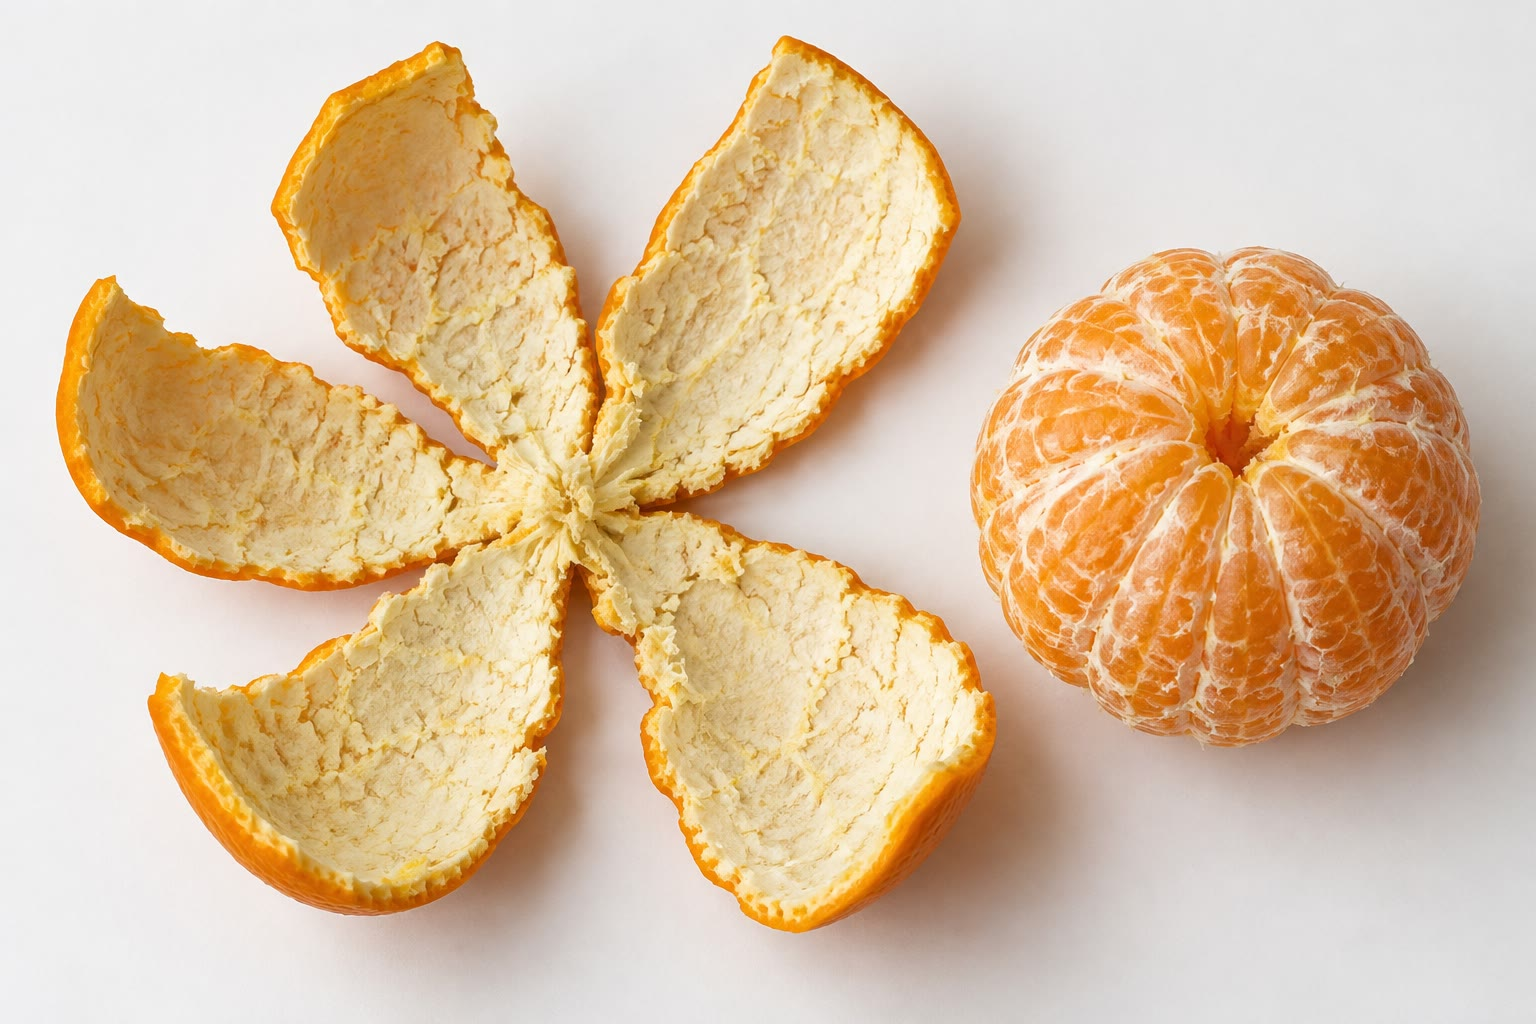
\includegraphics[width=0.4\linewidth]{images/book1/ai/g3-orange-peel.jpg}

{\small La piel de una naranja no puede quedar plana sin romperse.}
\end{omfigure}

\begin{remark}[El mapa y el globo no coinciden]\label{rem:g3:continents-and-oceans:disagree}
En este \omterm{def:g3:continents-and-oceans:world-map}{mapamundi}, la Antártida parece uno de los \omterm{def:g3:continents-and-oceans:continent}{continentes} más grandes,
estirada a lo largo de todo el borde de abajo. En el \omterm{def:g3:continents-and-oceans:globe}{globo terráqueo} es una
masa de tierra redonda, más pequeña que América del Sur. Cerca de los
\omterm{def:g3:continents-and-oceans:poles}{polos}, un mapa plano estira mucho la tierra. Cerca del \omterm{def:g3:continents-and-oceans:equator}{ecuador}, la estira
muy poco. Cuando quieras comparar el tamaño de dos lugares lejos del
\omterm{def:g3:continents-and-oceans:equator}{ecuador}, el \omterm{def:g3:continents-and-oceans:globe}{globo} dice la verdad.
\end{remark}

\begin{method}[Leer un mapamundi]\label{met:g3:continents-and-oceans:reading}
En un \omterm{def:g3:continents-and-oceans:world-map}{mapamundi} como este:
\begin{enumerate}
  \item el norte está arriba y el sur abajo; el \omterm{def:g3:continents-and-oceans:poles}{Polo Norte} es todo el borde
        de arriba y el \omterm{def:g3:continents-and-oceans:poles}{Polo Sur} todo el borde de abajo;
  \item el \omterm{def:g3:continents-and-oceans:equator}{ecuador} es la línea que cruza el centro: todo lo que está por
        encima está en el \omterm{def:g3:continents-and-oceans:equator}{hemisferio norte}, y todo lo que está por debajo,
        en el \omterm{def:g3:continents-and-oceans:equator}{hemisferio sur};
  \item los bordes izquierdo y derecho son la misma línea en el \omterm{def:g3:continents-and-oceans:globe}{globo}: un
        barco que sale por el borde derecho vuelve a entrar por el izquierdo.
\end{enumerate}
\end{method}

\section{Ejercicios}

\begin{exercise}[$\star$]\label{exo:g3:continents-and-oceans:1}
Nombra los siete \omterm{def:g3:continents-and-oceans:continent}{continentes}. ¿Cuál es el más grande? ¿Cuál es el más
pequeño?
\end{exercise}

\begin{exercise}[$\star$]\label{exo:g3:continents-and-oceans:2}
Nombra los cinco \omterm{def:g2:water-on-earth:ocean}{océanos}. ¿Cuál es el más grande? ¿Cuál es el más pequeño?
\end{exercise}

\begin{exercise}[$\star$]\label{exo:g3:continents-and-oceans:3}
Copia y completa con ``\omterm{def:g3:continents-and-oceans:poles}{Polo Norte}'', ``\omterm{def:g3:continents-and-oceans:poles}{Polo Sur}'' o ``\omterm{def:g3:continents-and-oceans:equator}{ecuador}'': el \dots{}
está arriba en un \omterm{def:g3:continents-and-oceans:globe}{globo terráqueo}; el \dots{} está abajo; el \dots{} da toda
la vuelta por el centro.
\end{exercise}

\begin{exercise}[$\star$]\label{exo:g3:continents-and-oceans:4}
¿\omterm{def:g3:continents-and-oceans:equator}{Hemisferio norte} o \omterm{def:g3:continents-and-oceans:equator}{hemisferio sur}? Europa; Australia; la Antártida;
América del Norte.
\end{exercise}

\begin{exercise}[$\star$]\label{exo:g3:continents-and-oceans:5}
¿Qué \omterm{def:g2:water-on-earth:ocean}{océano} rodea el \omterm{def:g3:continents-and-oceans:poles}{Polo Norte}? ¿Qué \omterm{def:g2:water-on-earth:ocean}{océano} rodea la Antártida?
\end{exercise}

\begin{exercise}[$\star\star$]\label{exo:g3:continents-and-oceans:6}
¿Qué \omterm{def:g2:water-on-earth:ocean}{océano} cruzas para ir de África a América del Sur? ¿Y de Australia a
América del Sur, yendo hacia el este? ¿Y de África a Australia?
\end{exercise}

\begin{exercise}[$\star\star$]\label{exo:g3:continents-and-oceans:7}
Sam vive en un país donde hace calor todo el año. Bo vive en una base
científica donde hiela todo el año. Uno de los dos vive cerca del \omterm{def:g3:continents-and-oceans:equator}{ecuador} y
el otro cerca de un \omterm{def:g3:continents-and-oceans:poles}{polo}. ¿Quién vive dónde?
\end{exercise}

\begin{exercise}[$\star\star$]\label{exo:g3:continents-and-oceans:8}
Lena hace girar el \omterm{def:g3:continents-and-oceans:globe}{globo terráqueo} 10 veces. Su dedo cae en el \omterm{def:g2:water-on-earth:ocean}{mar} 7 veces.
¿Cuántas veces cae en la tierra? ¿Es lo que esperabas? ¿Por qué?
\end{exercise}

\begin{exercise}[$\star\star$]\label{exo:g3:continents-and-oceans:9}
En el \omterm{def:g3:continents-and-oceans:world-map}{mapamundi} de la página~\pageref{fig:g3:continents-and-oceans:world-map},
el \omterm{def:g2:water-on-earth:ocean}{océano} Pacífico aparece dos veces. ¿Por qué? ¿Tiene la Tierra real dos
\omterm{def:g2:water-on-earth:ocean}{océanos} Pacíficos?
\end{exercise}

\begin{exercise}[$\star\star\star$]\label{exo:g3:continents-and-oceans:10}
Tom dice: ``En el \omterm{def:g3:continents-and-oceans:world-map}{mapamundi}, la Antártida es más larga que Asia, así que la
Antártida es el \omterm{def:g3:continents-and-oceans:continent}{continente} más grande''. ¿Tiene razón Tom? Usa la lista de
los \omterm{def:g3:continents-and-oceans:continent}{continentes} del más grande al más pequeño, y di por qué el \omterm{def:g3:continents-and-oceans:world-map}{mapamundi} le
engaña.
\end{exercise}
